\documentclass[a4paper,12pt]{article}
\usepackage[super,numbers,sort&compress]{natbib}
%\PassOptionsToPackage{numbers, compress}{natbib}
\usepackage{geometry}
 \geometry{
	a4paper,
	left=1in,
	right=1in,
	top=1in,
	bottom=1in,
}
\headsep=0.25in
\usepackage{graphicx}
\usepackage{amsmath}
\usepackage{amssymb}
\usepackage{multirow}
\usepackage{booktabs}
\usepackage{hyperref}
\newcommand{\bd}[1]{\mathbf{#1}}
\newcommand{\pathexpr}[3]{{#1}_{#2}^{(#3)}}
\newcommand{\ttt}[1]{\texttt{#1}}
\newcommand{\grad}[2]{\nabla_{\bd{#2}} #1}
\newcommand{\hess}[1]{\bd{H}_{\bd{#1}}}

\makeatletter 
\renewcommand\@biblabel[1]{#1.}
\makeatother

%\bibliographystyle{plain}
\bibliographystyle{unsrt}
\title{
	\vspace{4in}
	\textmd{\bf Supplementary Materials}\\
	\vspace{3in}
}
\date{}
\begin{document}
	\maketitle
	\thispagestyle{empty}
	\newpage
	\setcounter{page}{1}
	\section*{Appendix A. Calculation of gradient and Hessian matrix} \label{sec:calcu}
	In this section, we provide close form expressions for calculation of the gradients $\grad{L}{F}$ and Hessian matrices $\hess{F}$ for classification and survival model, as needed in Section 2.1 in the main text.
	
	\noindent $\bullet$ Classification model:
	\begin{eqnarray*}
		(\grad{L}{F})_i & = & \frac{\partial L(\bd{y}, \bd{F})}{\partial F(\bd{x}_i, \bd{z}_i)} = -\frac{y_i}{1+\exp[y_i F(\bd{x}_i, \bd{z}_i)]} \\
		(\hess{F})_{ij} & = & \frac{\partial^2 L(\bd{y}, \bd{F})}{\partial F(\bd{x}_i, \bd{z}_i) \partial F(\bd{x}_j, \bd{z}_j)} \\
		& = & \begin{cases}
			\frac{\exp[y_iF(\bd{x}_i, \bd{z}_i]}{(1+\exp[y_iF(\bd{x}_i, \bd{z}_i)])^2} &\text{if  $i = j$}\\
			0 &\text{if $i \neq j$}
		\end{cases}
	\end{eqnarray*}
	\noindent $\bullet$ Survival model:
	\begin{eqnarray*}
		(\grad{L}{F})_i &=&   \frac{\partial L(\bd{y}, \bd{F})}{\partial F(\bd{x}_i, \bd{z}_i)}  = -\frac{1}{N}\left( \delta_i - \sum^N_{j=1}\delta_j1_{\left\lbrace t_i \geq t_j\right\rbrace }\frac{\exp[F(\bd{x}_i, \bd{z}_i)]}{\sum^N_{r=1}1_{\left\lbrace t_r \geq t_j \right\rbrace }\exp[F(\bd{x}_r, \bd{z}_r)]}\right) \\
		(\hess{F})_{ij} & = & \frac{\partial^2 L(\bd{y}, \bd{F})}{\partial F(\bd{x}_i, \bd{z}_i) \partial F(\bd{x}_j, \bd{z}_j)} \\
		& = &  \frac{1}{N} \sum^N_{l=1}\delta_j 1_{\left\lbrace t_i \geq t_l\right\rbrace }  \frac{1_{\{ i = j\}}\exp[F(\bd{x}_i, \bd{z}_i)]}{ \sum^N_{r=1}1_{\left\lbrace t_r \geq t_l \right\rbrace }\exp[F(\bd{x}_r, \bd{z}_r)]} - \\
		& & \frac{1}{N} \sum^N_{l=1}\delta_j 1_{\left\lbrace t_i \geq t_l\right\rbrace } 1_{\left\lbrace t_j \geq t_l \right\rbrace }\frac{\exp[F(\bd{x}_i, \bd{z}_i)]\exp[F(\bd{x}_j, \bd{z}_j)]}{\left( \sum^N_{r=1}1_{\left\lbrace t_r \geq t_l \right\rbrace }\exp[F(\bd{x}_r, \bd{z}_r)]\right) ^2} 
	\end{eqnarray*}
	
	
	Since the regression model's loss function is quadratic itself, we do not need to calculate the gradient or Hessian matrix to make approximation. As a result of using the negative log partial likelihood as loss in survival model, the loss for each sample is dependent on the $F(\bd{x}, \bd{z})$ values of other samples, which leads to non-zero off-diagonal values in the Hessian matrix. It is more complex as compared to the diagonal Hessian matrix in classification problem, and therefore causing the algorithm to be slower than classification as well.
	\newpage
	\section*{Appendix B. Proof of the reduction to LASSO and Ridge Regression} \label{sec:proof}
	In this section, we prove the following result about Equation (3) as stated in Section 2.1:
	
	By applying transformation
	\begin{eqnarray*}
		\tilde{\eta} &=& \frac{1}{\sqrt{2}}\hess{F}^{\frac{1}{2}}(I_N - Z(Z^T \hess{F} Z)^{-1}Z^T \hess{F})\hess{F}^{-1}\grad{L}{F}\\
		\tilde{K}_m &=& \frac{1}{\sqrt{2}}\hess{F}^{\frac{1}{2}}(I_N - Z(Z^T\hess{F}Z)^{-1}Z^T\hess{F})K_m,
	\end{eqnarray*}
	solving $\beta$ in Equation (3) is reduced to a penalized linear regression problem
	\begin{equation*}
	\min_{\beta} \|\tilde{\eta} + \tilde{K}_m \beta \|_2^2 + \lambda \Omega(f).
	\end{equation*}
	
	Because the penalty term $\Omega(f)$ in Equation (3) does not involve $\gamma$, we can fix $\beta$ and solve $\gamma$ as a weighted least square problem:
	$$\gamma = -(Z^T\hess{F}Z)^{-1}Z^T\hess{F}(K_m\beta + \hess{F}^{-1}\grad{L}{F})$$
	Plugging it back to Equation (3), we can get the following reduction:
	\begin{eqnarray*}
		& & \min_{\beta, \gamma} \frac{1}{2} (K_m \beta + Z \gamma + \hess{F}^{-1} \grad{L}{F})^T \hess{F} (K_m \beta + Z \gamma + \hess{F}^{-1} \grad{L}{F}) + \lambda \Omega(f) \\
		& = & \min_{\beta} \frac{1}{2} [ U(K_m \beta + \hess{F}^{-1} \grad{L}{F}) ]^T \hess{F} [ U (K_m \beta + \hess{F}^{-1} \grad{L}{F}) ]  + \lambda \Omega(f) \\
		& = & \min_{\beta}  \| \frac{1}{\sqrt{2}}\hess{F}^{\frac{1}{2}}U(K_m \beta + \hess{F}^{-1} \grad{L}{F}) \|_2^2+ \lambda \Omega(f) \\
		&=& \min_{\beta} \|\tilde{\eta} + \tilde{K}_m \beta \|_2^2 + \lambda \Omega(f), 
	\end{eqnarray*}
	which proves our statement. In the equations, the matrix $U = (I_N -Z(Z^T\hess{F}Z)^{-1}Z^T\hess{F})$, is an intermediate matrix.
	
	\newpage
	\section*{Appendix C. Calculation of C-index}
	\label{sec:Cind}
	In this section, we describe the calculation of C-index for evaluation of survival prediction accuracy. For each pair of samples, assume they have survival outcomes $(t_i, \delta_i)$ and $(t_j, \delta_j)$, and estimated risk scores $f_i$ and $f_j$. The concordance for the pair is calculated as follows:
	\begin{itemize}
		\item If the sample with smaller $t$ is censored, omit the pair
		\item If $t_i = t_j$ and both samples are censored, omit the pair
		\item If $t_i \neq t_j$\\
		\qquad - If  $f_i = f_j$, concordance equals to 0.5\\
		\qquad - If the sample with higher risk has smaller $t$, then concordance equals to 1, otherwise 0
		\item If $t_i = t_j$\\
		\qquad - If $\delta_i = \delta_j = 1$, concordance equals to 1 if $f_i = f_j$, otherwise 0.5\\
		\qquad - If the censored sample has smaller risk score, concordance is 1, otherwise 0
		
	\end{itemize}
	We look at all pairs of samples, and the C-index is defined as
	$$\text{C-index} = \frac{ \text{Total Concordance} }{\# \text{Permissible pairs} }$$
	\newpage
	\section*{Appendix D. Parameter tuning}
	\label{sec:tune}
	The usage of most methods in this article involves tuning of certain model parameters. In general, we generated a series of candidate values for each parameter, and considered all possible combinations among them. Cross-validation was utilized to determine the optimal combination and corresponding prediction accuracy.
	
	\begin{itemize}
		\item PKB\\
		In simulations, we used the following candidate values for tuning parameters:\\
		1. kernel function: radial basis function (rbf), polynomial kernel with degree 3 (poly3)\\
		2. learning rate: 0.01, 0.05\\
		3. penalty multiplier: 0.04, 0.2, 1\\
		An automatic procedure is proposed in Zeng et al\cite{zeng2019pathway} to determine the penalty parameter, but it is often overly strong. Therefore, we tried the penalty multipliers above ($\leq 1$) to soften the penalty term. In real data applications, we used the following candidate values:\\
		1. kernel function: rbf, poly3\\
		2. learning rate: 0.005, 0.03\\
		3. penalty multiplier: 0.04, 0.2, 1\\
		4. pathway databases: KEGG, Biocarta, GO-BP
		
		\item LASSO/ Ridge Regression/ Elastic Net\\
		The LASSO solver in python \ttt{sklearn} module has a default method for generating a series of feasible penalty parameters $\lambda$. We used it to generate 100 $
		\lambda$s and evaluated prediction performances through cross-validation. The optimal value was used for prediction.\\
		For Ridge Regression, we used 100 values between 0.1 and 1,000 (equally spaced on log scale) as candidate penalty parameters. The value demonstrating the optimal prediction performance in cross-validation was used to predict test data.\\
		The Elastic Net method has penalty term $ r \alpha \|\beta\|_1 + (1-r)\alpha/2 \|\beta\|^2_2$, which involves two tuning parameters, $r$ and $\alpha$. $\alpha$ can be considered as the total penalty, and $r$ determines how much of it is assigned to the $L_1$ part. In our parameter tuning, we considered all combinations of $r = 0.1, 0.2, \ldots, 1$ and 30 $\alpha$ values generated by default.
		
		\item RandomForest\\
		We tuned the parameters, number of trees and maximum depth for a single tree, for optimized prediction performance. We had a list of candidate values for each parameter, and fit prediction models using all possible parameter value combinations. Results for the optimal combination were reported. The candidate values we used for both parameters are as follows:\\
		1. number of trees in forest: 500 and 800\\
		2. maximum tree depth: 3, 5, 7, and no constraint
		\item Gradient Boosting Regression\\
		The tuning parameters are: maximum tree depth and learning rate. The tuning process is similar to the procedure in RandomForest. For each parameter combination, we used out-of-bag (OOB) samples (1/3 of training data in each iteration) to decide optimal number of iterations, and used the optimal iteration number to fit a model without OOB sample. The candidate values for tuning parameters are:\\
		1. maximum tree depth: 3, 5, and 7\\
		2. learning rate: 0.002, 0.01, and 0.05
		\item SVR\\
		We tuned three parameters of SVR: $C$, which adjusts the penalty on samples violating the $\epsilon$-tube; $\epsilon$, which is the width of the $\epsilon$-tube; and the kernel functions. The candidate values for these parameters are:\\
		1. $C$: 10 values equally spaced on log scale between 0.1 and 1000\\
		2. $\epsilon$: 10 values equally spaced between 0.1 and 4\\
		3. kernel functions: rbf, poly2, and poly3
		
		\item Glmnet\\
		The parameters we tuned for Glmnet included:  $\alpha \in (0, 1)$, which is the ElasticNet mixing parameter, determining the fraction of $L_1$ penalty; $\lambda$, which adjusts the overall strength of the penalty. Candidate values for them are:\\
		1.	$\alpha$: 20 values equally spaced between 0 and 1\\
		2.	$\lambda$: 0.001, 0.01, 0.1, 1, 2, 5, and 10
		\item RandomSurvivalForest\\
		We tuned the parameters including the splitting rule of the trees, the number of trees, and the depth of the trees. Candidate values for the parameters are:\\
		1.	Splitting rules: logrank (splitting nodes by maximization of the log-rank test statistic), and logrankscore (splitting nodes by maximization of the standardized log-rank statistic)\\
		2.	The number of trees: 100, 200, and 500\\
		3.	The maximum tree depth: 3, 5, and 7
		
		\item CoxBoost\\
		The tuning parameters for CoxBoost were step-size factor, which determined the step-size modification factor by which each boosting step size should be changed; and the number of iterations, which controlled the total number of boosting steps. \\
		1.	Step-size factor: 0.01, 0.1, 0.5, 1, and 2\\
		2.	The number of boosting iterations: 100, 250, and 500 
	\end{itemize}
\newpage
\section*{Appendix E. Pathway enrichment analysis in TCGA survival datasets}\label{sec:gsea}
The pathway enrichment analysis was performed based on the following steps:
\begin{itemize}
	\item[1.] For each gene, we performed a Cox regression using the clinical features and the gene's expression as predictors. P-values for each gene were calculated from the Cox models.
	\item[2.] We chose $20\%$ genes with the smallest p-values as relevant genes to patients' survival times. 
	\item[3.] The relevant genes were used to perform Fisher's exact test-based enrichment analysis \cite{huang2008bioinformatics} on the pathway database (KEGG, GO-BP, or Biocarta) used in the PKB model that achieved the highest accuracy. An enrichment p-value was calculated for each pathway.
\end{itemize}

\begin{figure}[htp]
	\centering
	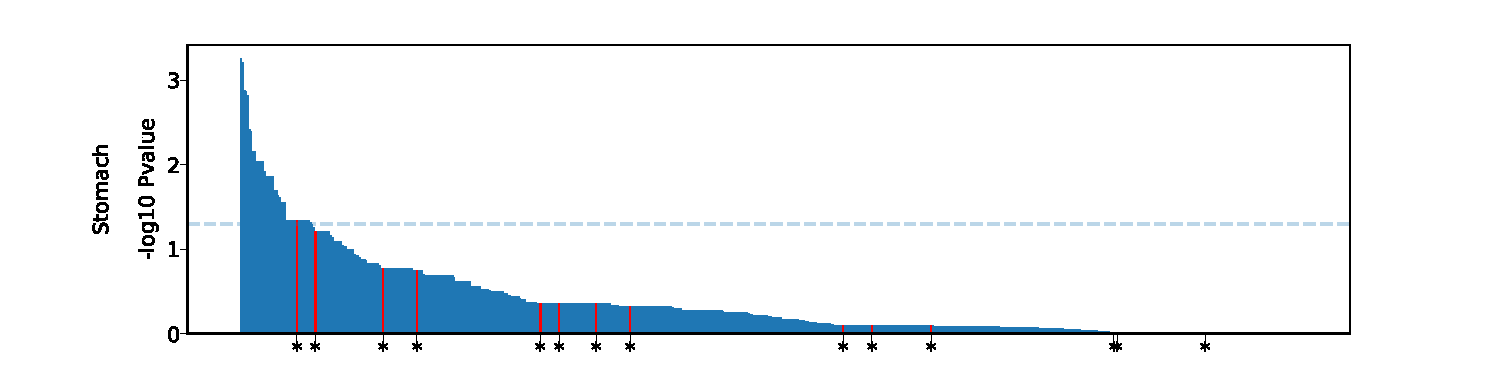
\includegraphics[width=\textwidth]{GSEA_Stomach.pdf}\\ \vspace{-3mm}
	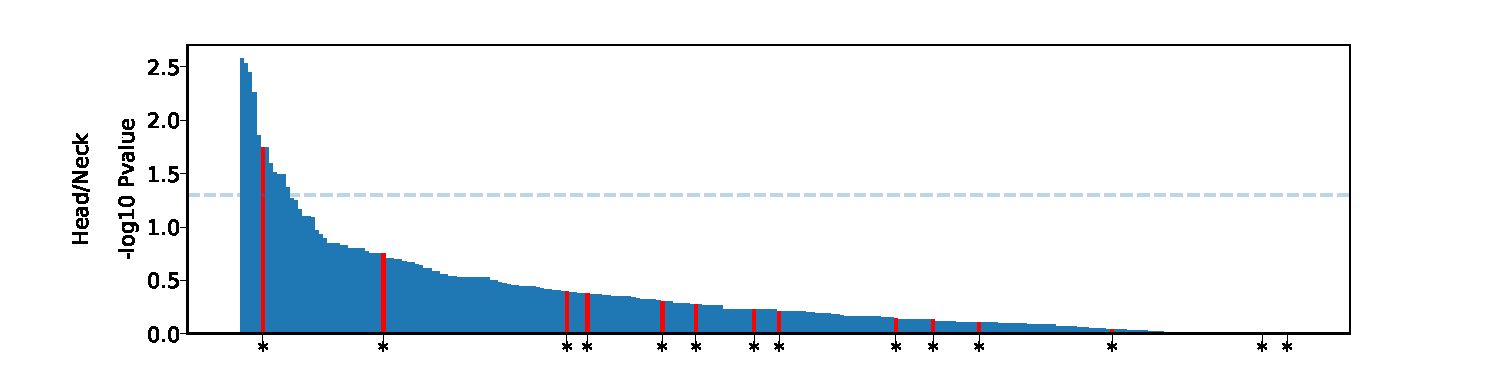
\includegraphics[width=\textwidth]{GSEA_Head_Neck.pdf}\\ \vspace{-3mm}
	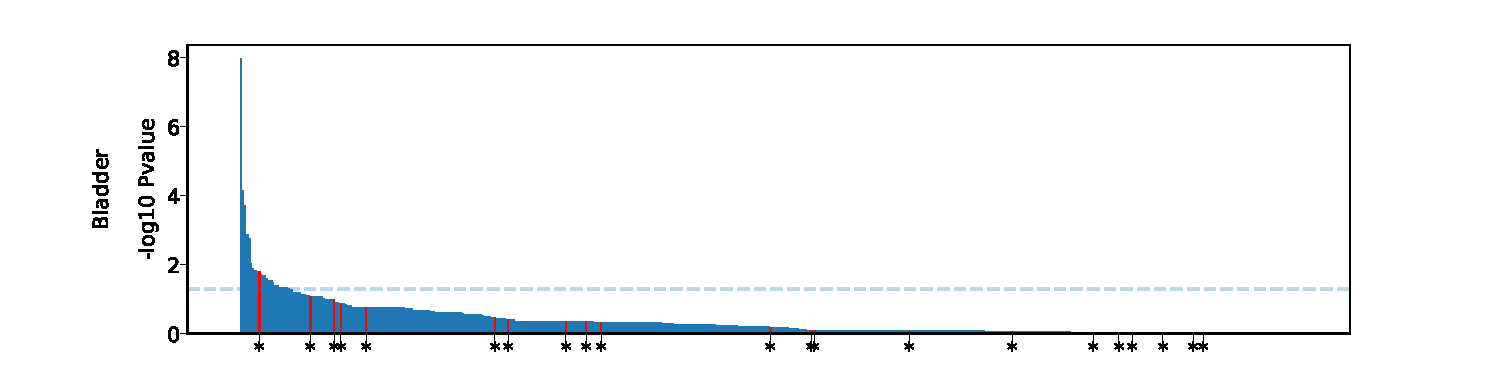
\includegraphics[width=\textwidth]{GSEA_Bladder.pdf}\\ \vspace{-3mm}
	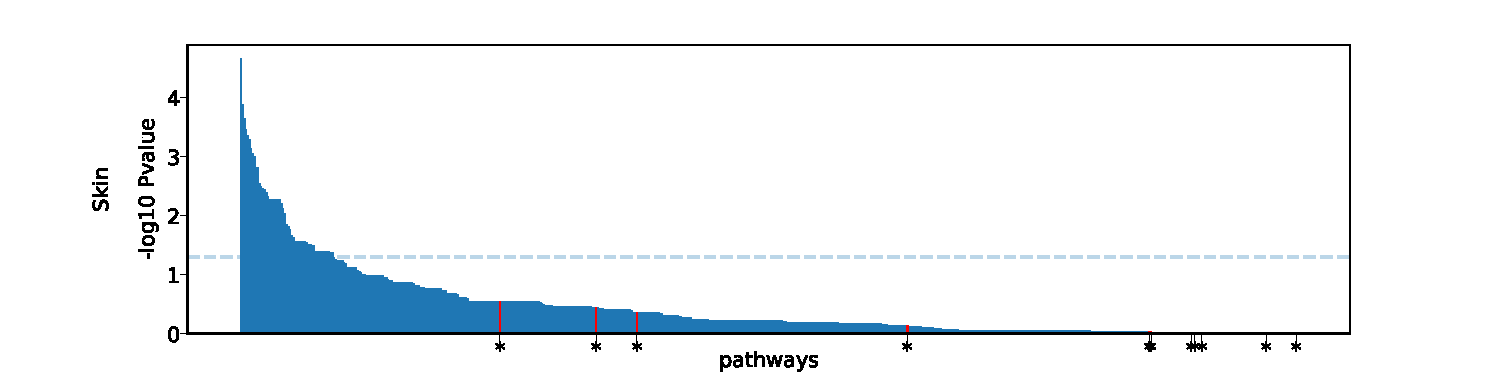
\includegraphics[width=\textwidth]{GSEA_Skin.pdf}
	\caption{Enrichment analysis on stomach, head/neck, bladder, and skin cancer datasets. X-axis represents pathways sorted by their p-values in the enrichment analysis. The blue dashed line corresponds to p-value 0.05. The pathways marked with red bars and stars are pathways with significant weights in PKB.}
\end{figure}
\newpage
\section*{Appendix F. PKB model pathway weights from survival simulations}
\label{sec:surv_weights}
\begin{figure}[htp]
	\centering
	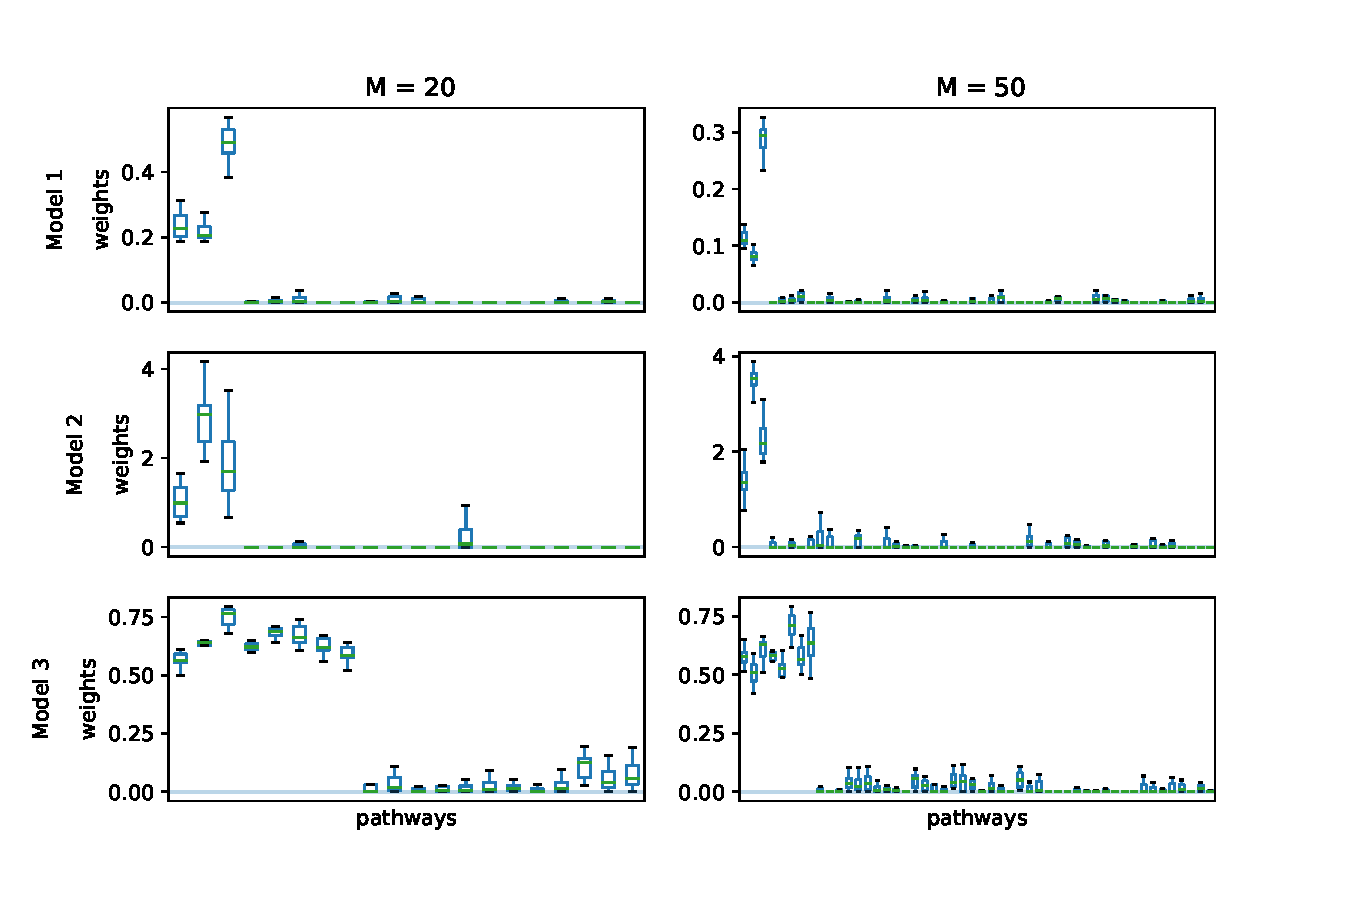
\includegraphics[width=1\textwidth]{simu_surv_weights.pdf}
	\caption{Boxplots for pathway weights in the survival simulations. Each box represents the weights distribution for one pathway over ten PKB runs.}
\end{figure}
\newpage
\section*{Appendix G. Weighted PKB prediction results}
\label{sec:weightedPKB}

\begin{figure}[htp]
	\centering
	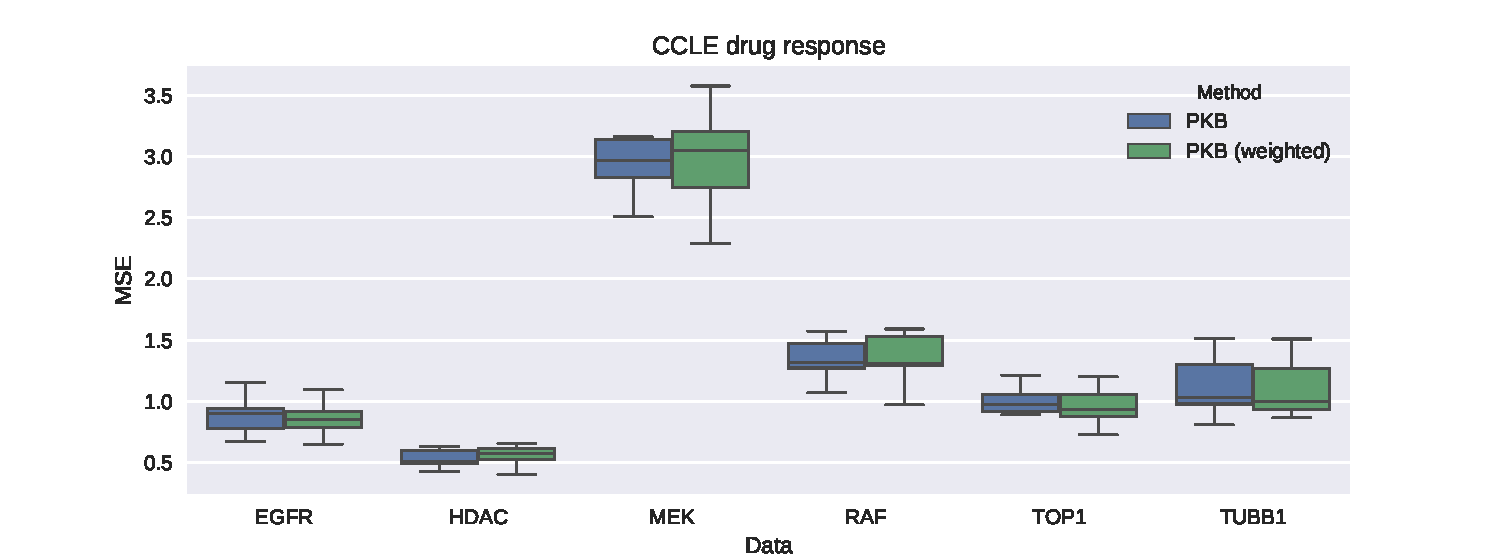
\includegraphics[width=1\textwidth]{reg_W_vs_noW.pdf}\\ \vspace{-3mm}
	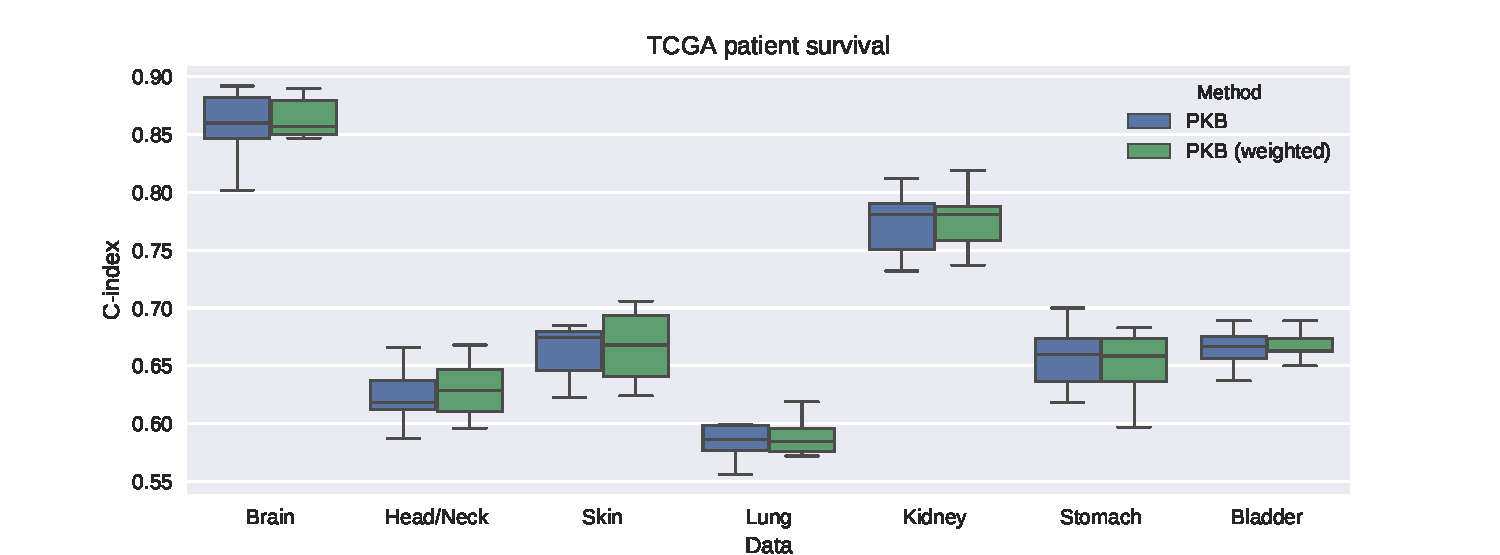
\includegraphics[width=1\textwidth]{surv_W_vs_noW.pdf}
	\caption{Prediction performances from PKB and PKB with gene weights. The upper panel demonstrates prediction MSEs from CCLE drug response datasets. The lower panel demonstrates prediction C-index from TCGA patient survival datasets. No significant difference in accuracy can be observed from the two methods.}
\end{figure}
\newpage
\section*{Appendix H. Standard deviations for the prediction accuracy measures in simulations and real data appications}
\label{sec:std}

% Please add the following required packages to your document preamble:
% \usepackage{multirow}
\begin{table}[htp]
	\centering
	\begin{tabular}{lllllllll}
		\hline
		\multirow{2}{*}{Method} & \multicolumn{2}{c}{Model 1} &  & \multicolumn{2}{c}{Model 2} &  & \multicolumn{2}{c}{Model 3} \\ \cline{2-3} \cline{5-6} \cline{8-9} 
		& M = 20       & M = 50       &  & M = 20       & M = 50       &  & M = 20       & M = 50       \\ \hline
		PKB-$L_1$                  & 2.02         & 7.63         &  & 5.73         & 4.26         &  & 0.95         & 0.77         \\
		PKB-$L_2$                & 2.09         & 6.67         &  & 5.34         & 3.93         &  & 0.59         & 0.58         \\
		LASSO                   & 4.21         & 11.35        &  & 5.91         & 8.84         &  & 1.81         & 2.2          \\
		Ridge                   & 3.81         & 13.03        &  & 8.46         & 9.42         &  & 1.81         & 2.19         \\
		ElasticNet              & 4.17         & 10.64        &  & 6.08         & 8.4          &  & 2.05         & 2.43         \\
		RandomForest            & 4.2          & 14.51        &  & 7.38         & 10.43        &  & 1.54         & 2.03         \\
		GBR                     & 4.96         & 12.53        &  & 8.08         & 10.21        &  & 1.72         & 1.8          \\
		SVR                     & 3.61         & 13.16        &  & 8.08         & 9.46         &  & 1.28         & 1.84         \\ \hline
	\end{tabular}
	\caption{Standard deviations for prediction MSE in regression simulation studies.}
\end{table}


% Please add the following required packages to your document preamble:
% \usepackage{multirow}
\begin{table}[htp]
	\centering
	\begin{tabular}{lllllllll}
		\hline
		\multirow{2}{*}{Method} & \multicolumn{2}{c}{Model 1} & \multicolumn{1}{c}{} & \multicolumn{2}{c}{Model 2} & \multicolumn{1}{c}{} & \multicolumn{2}{c}{Model 3} \\ \cline{2-3} \cline{5-6} \cline{8-9} 
		& M = 20       & M = 50       &                      & M = 20       & M = 50       &                      & M = 20       & M = 50       \\ \hline
		PKB-$L_1$                  & 0.01         & 0.02         &                      & 0.03         & 0.03         &                      & 0.01         & 0.01         \\
		PKB-$L_2$                  & 0.01         & 0.02         &                      & 0.04         & 0.05         &                      & 0.01         & 0.01         \\
		Glmnet                  & 0.02         & 0.02         &                      & 0.02         & 0.01         &                      & 0.02         & 0.01         \\
		RandomSurvivalForest    & 0.03         & 0.03         &                      & 0.03         & 0.03         &                      & 0.03         & 0.03         \\
		CoxBoost                & 0.02         & 0.02         &                      & 0.03         & 0.02         &                      & 0.02         & 0.02         \\ \hline
	\end{tabular}
	\caption{Standard deviations for prediction C-index in survival simulation studies.}
\end{table}

\newpage

\begin{table}[htp]
	\centering
	\begin{tabular}{lllllll}
		\hline
		Method       & EGFR & HDAC & MEK  & RAF  & TOP1 & TUBB1 \\ \hline
		PKB-$L_1$       & 0.14 & 0.07 & 0.27 & 0.14 & 0.13 & 0.23  \\
		PKB-$L_2$       & 0.14 & 0.07 & 0.28 & 0.14 & 0.14 & 0.22  \\
		LASSO        & 0.2  & 0.08 & 0.62 & 0.2  & 0.13 & 0.21  \\
		Ridge        & 0.14 & 0.07 & 0.35 & 0.29 & 0.15 & 0.23  \\
		ElasticNet   & 0.16 & 0.09 & 0.51 & 0.18 & 0.13 & 0.21  \\
		RandomForest & 0.12 & 0.08 & 0.24 & 0.18 & 0.13 & 0.21  \\
		GBR          & 0.14 & 0.08 & 0.27 & 0.14 & 0.13 & 0.23  \\
		SVR          & 0.13 & 0.08 & 0.31 & 0.14 & 0.13 & 0.23  \\ \hline
	\end{tabular}
	\caption{Standard deviations for prediction MSE in CCLE drug response datasets.}
\end{table}

\begin{table}[htp]
	\centering
	\begin{tabular}{llllllll}
		\hline
		Method               & Brain & Head/Neck & Skin & Lung & Kidney & Stomach & Bladder \\ \hline
		PKB-$L_1$               & 0.03  & 0.02 & 0.02     & 0.03 & 0.03   & 0.03    & 0.02    \\
		PKB-$L_2$               & 0.03  & 0.03 & 0.03     & 0.03 & 0.02   & 0.02    & 0.02    \\
		Glmnet               & 0.02  & 0.02 & 0.02     & 0.01 & 0.01   & 0.03    & 0.03    \\
		RandomSurvivalForest & 0.02  & 0.02 & 0.02     & 0.01 & 0.02   & 0.02    & 0.03    \\
		CoxBoost             & 0.02  & 0.01 & 0.02     & 0.02 & 0.02   & 0.03    & 0.02    \\ \hline
	\end{tabular}
	\caption{Standard deviations for prediction C-index in TCGA patient survival datasets.}
\end{table}
	\newpage
	\bibliography{mybib_DB}
	\end{document}